\documentclass[a4paper,14pt]{extreport} % формат документа

\usepackage{amsmath}
\usepackage{cmap} % поиск в ПДФ
\usepackage[T2A]{fontenc} % кодировка
\usepackage[utf8]{inputenc} % кодировка исходного текста
\usepackage[english,russian]{babel} % локализация и переносы
\usepackage[left = 2cm, right = 1cm, top = 2cm, bottom = 2 cm]{geometry} % поля
\usepackage{listings}
\usepackage{graphicx} % для вставки рисунков
\usepackage{amsmath}
\usepackage{float}
\usepackage{multirow}
\graphicspath{{pictures/}}
\DeclareGraphicsExtensions{.pdf,.png,.jpg}
\newcommand{\anonsection}[1]{\section*{#1}\addcontentsline{toc}{section}{#1}}

\lstset{ %
	language=python,                % Язык программирования 
	numbers=left,                   % С какой стороны нумеровать          
	frame=single,                    % Добавить рамку
	escapebegin=\begin{russian}\commentfont,
    escapeend=\end{russian},
    literate={Ö}{{\"O}}1
    {Ä}{{\"A}}1
    {Ü}{{\"U}}1
    {ß}{{\ss}}1
    {ü}{{\"u}}1
    {ä}{{\"a}}1
    {ö}{{\"o}}1
    {~}{{\textasciitilde}}1
    {а}{{\selectfont\char224}}1
    {б}{{\selectfont\char225}}1
    {в}{{\selectfont\char226}}1
    {г}{{\selectfont\char227}}1
    {д}{{\selectfont\char228}}1
    {е}{{\selectfont\char229}}1
    {ё}{{\"e}}1
    {ж}{{\selectfont\char230}}1
    {з}{{\selectfont\char231}}1
    {и}{{\selectfont\char232}}1
    {й}{{\selectfont\char233}}1
    {к}{{\selectfont\char234}}1
    {л}{{\selectfont\char235}}1
    {м}{{\selectfont\char236}}1
    {н}{{\selectfont\char237}}1
    {о}{{\selectfont\char238}}1
    {п}{{\selectfont\char239}}1
    {р}{{\selectfont\char240}}1
    {с}{{\selectfont\char241}}1
    {т}{{\selectfont\char242}}1
    {у}{{\selectfont\char243}}1
    {ф}{{\selectfont\char244}}1
    {х}{{\selectfont\char245}}1
    {ц}{{\selectfont\char246}}1
    {ч}{{\selectfont\char247}}1
    {ш}{{\selectfont\char248}}1
    {щ}{{\selectfont\char249}}1
    {ъ}{{\selectfont\char250}}1
    {ы}{{\selectfont\char251}}1
    {ь}{{\selectfont\char252}}1
    {э}{{\selectfont\char253}}1
    {ю}{{\selectfont\char254}}1
    {я}{{\selectfont\char255}}1
    {А}{{\selectfont\char192}}1
    {Б}{{\selectfont\char193}}1
    {В}{{\selectfont\char194}}1
    {Г}{{\selectfont\char195}}1
    {Д}{{\selectfont\char196}}1
    {Е}{{\selectfont\char197}}1
    {Ё}{{\"E}}1
    {Ж}{{\selectfont\char198}}1
    {З}{{\selectfont\char199}}1
    {И}{{\selectfont\char200}}1
    {Й}{{\selectfont\char201}}1
    {К}{{\selectfont\char202}}1
    {Л}{{\selectfont\char203}}1
    {М}{{\selectfont\char204}}1
    {Н}{{\selectfont\char205}}1
    {О}{{\selectfont\char206}}1
    {П}{{\selectfont\char207}}1
    {Р}{{\selectfont\char208}}1
    {С}{{\selectfont\char209}}1
    {Т}{{\selectfont\char210}}1
    {У}{{\selectfont\char211}}1
    {Ф}{{\selectfont\char212}}1
    {Х}{{\selectfont\char213}}1
    {Ц}{{\selectfont\char214}}1
    {Ч}{{\selectfont\char215}}1
    {Ш}{{\selectfont\char216}}1
    {Щ}{{\selectfont\char217}}1
    {Ъ}{{\selectfont\char218}}1
    {Ы}{{\selectfont\char219}}1
    {Ь}{{\selectfont\char220}}1
    {Э}{{\selectfont\char221}}1
    {Ю}{{\selectfont\char222}}1
    {Я}{{\selectfont\char223}}1
    {і}{{\selectfont\char105}}1
    {ї}{{\selectfont\char168}}1
    {є}{{\selectfont\char185}}1
    {ґ}{{\selectfont\char160}}1
    {І}{{\selectfont\char73}}1
    {Ї}{{\selectfont\char136}}1
    {Є}{{\selectfont\char153}}1
    {Ґ}{{\selectfont\char128}}1
}

\begin{document}
\begin{titlepage}

    \begin{table}[H]
        \centering
        \footnotesize
        \begin{tabular}{cc}
            \multirow{8}{*}{
\includegraphics[scale=0.35]{bmstu.jpg}}
            & \\
            & \\
            & \textbf{Министерство науки и высшего образования Российской Федерации} \\
            & \textbf{Федеральное государственное бюджетное образовательное учреждение} \\
            & \textbf{высшего образования} \\
            & \textbf{<<Московский государственный технический} \\
            & \textbf{университет имени Н.Э. Баумана>>} \\
            & \textbf{(МГТУ им. Н.Э. Баумана)} \\
        \end{tabular}
    \end{table}

    \vspace{-2.5cm}

    \begin{flushleft}
        \rule[-1cm]{\textwidth}{3pt}
        \rule{\textwidth}{1pt}
    \end{flushleft}

    \begin{flushleft}
        \small
        ФАКУЛЬТЕТ
        \underline{<<Информатика и системы управления>>\ \ \ \ \ \ \ 
        \ \ \ \ \ \ \ \ \ \ \ \ \ \ \ \ \ \ \ \ \ \ \ \ \ \ \ \ \ \ \ 
    \ \ \ \ \ \ \ \ \ \ \ \ \ \ \ } \\
        КАФЕДРА
        \underline{<<Программное обеспечение ЭВМ и
        информационные технологии>>
        \ \ \ \ \ \ \ \ \ \ \ \ \ \ \ \ \ \ \ \ }
    \end{flushleft}

    \vspace{2cm}

    \begin{center}
        \textbf{Лабораторная работа № 5} \\
        \vspace{0.5cm}
    \end{center}

    \vspace{4cm}

    \begin{flushleft}
        \begin{tabular}{ll}
            \textbf{Дисциплина} & Моделирование.  \\
            \textbf{Тема} & Исследование математической модели на основе \\
            & технологии вычислительного эксперимента \\
            \\
            \textbf{Студент} & Сиденко А.Г. \\
            \textbf{Группа} & ИУ7-63Б \\
            \textbf{Оценка (баллы)} & \\
            \textbf{Преподаватель} & Градов В.М.   \\
        \end{tabular}
    \end{flushleft}

    \vspace{4cm}

   \begin{center}
        Москва, 2020 г.
    \end{center}

\end{titlepage}

\textbf{Цель работы:} Получение навыков проведения исследований компьютерной математической модели, построенной на квазилинейном уравнении параболического типа. Исследование проводится  с помощью программы, созданной в лабораторной работе №4. 

Все величины как в лабораторной 4, кроме

$$F(t)=\frac{F_{max}}{t_{max}}t \cdot exp\bigg(-\bigg(\frac{t}{t_{max}}-1\bigg)\bigg)$$

где

$F_{max}$ -- амплитуда импульса потока 

$t_{max}$ -- время достижения амплитуды

\hfill

\textbf{Результаты}


\begin{enumerate}
\item Провести исследование по выбору оптимальных шагов по времени и пространству. Шаги должны быть максимально большими при сохранении устойчивости разностной схемы и заданной точности расчета. 

Точность расчета будем оценивать, уменьшая шаги и наблюдая сходимость решений, как это делалось в лабораторной работе №1. 

\textbf{Шаг по пространству:}

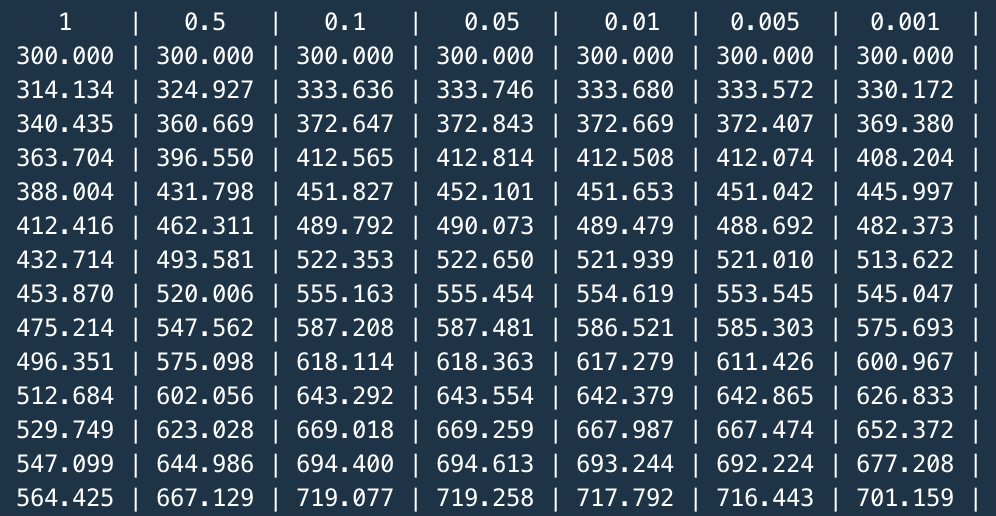
\includegraphics{1}

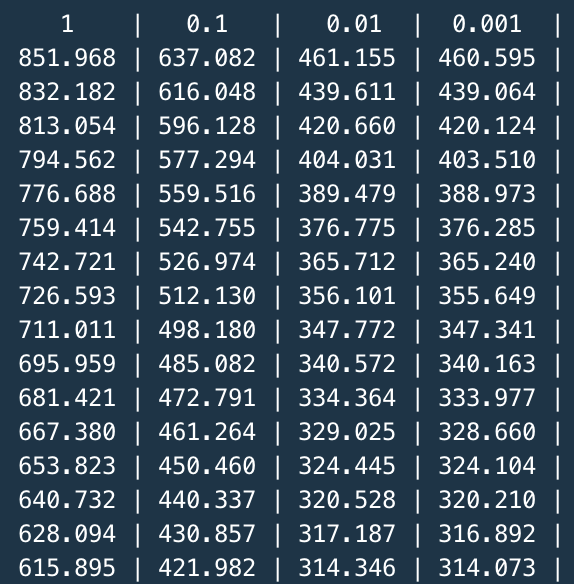
\includegraphics{2}

Таким образом, оптимальный шаг $h=0.1$. 

\textbf{Шаг по времени:}

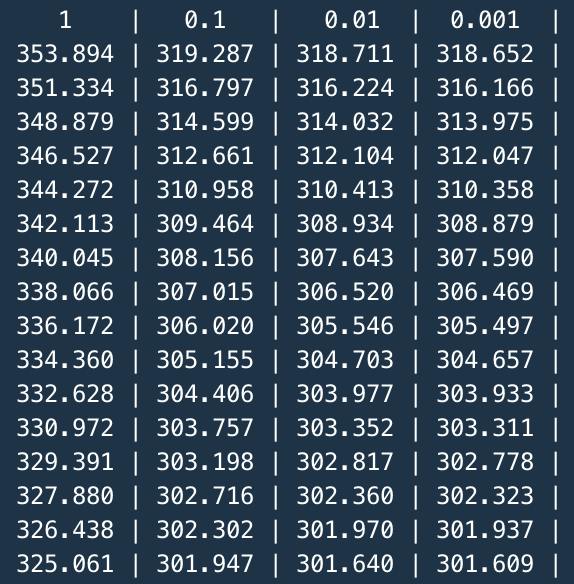
\includegraphics{3}

Таким образом, оптимальный шаг $\tau=0.1$. 

\newpage

Рассмотрим влияние на получаемые результаты амплитуды импульса  и  времени. 

$F_{max}=100$

$t_{max}=10$ 

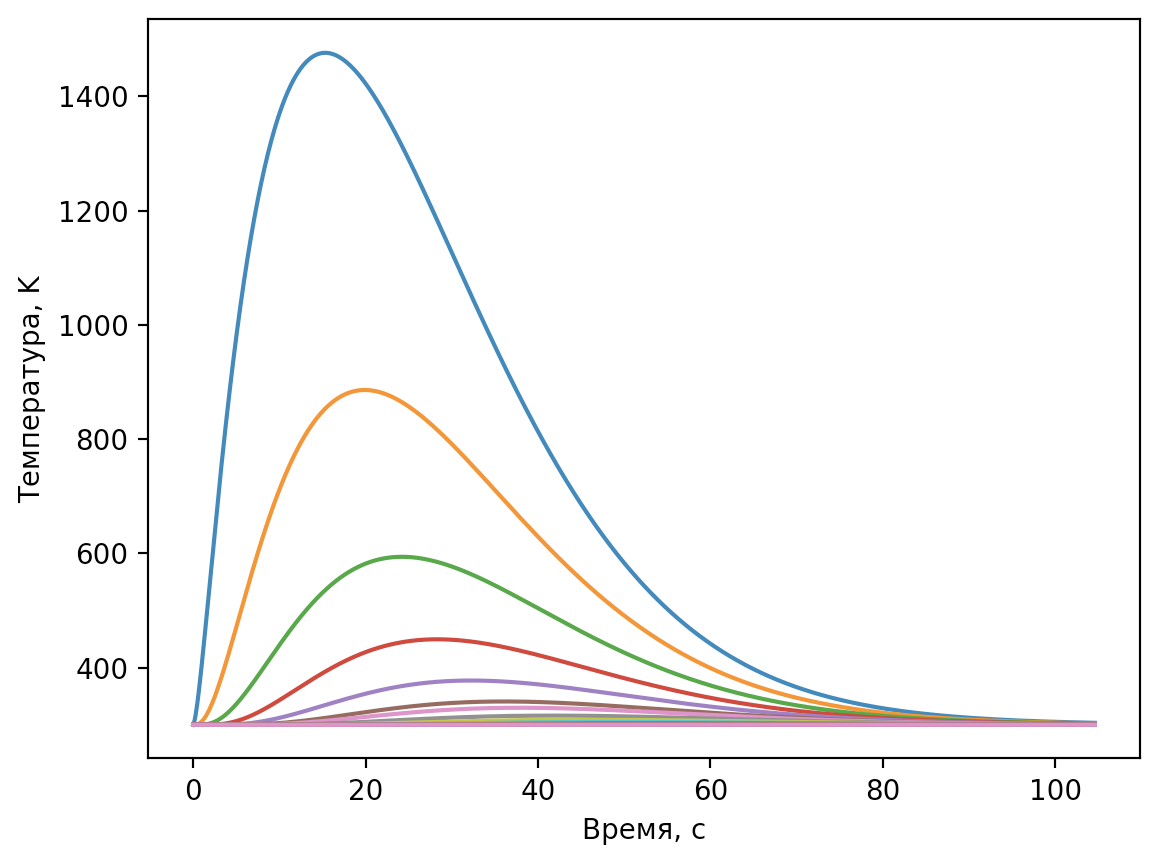
\includegraphics[scale=0.6]{4}

$F_{max}=1000$

$t_{max}=10$ 

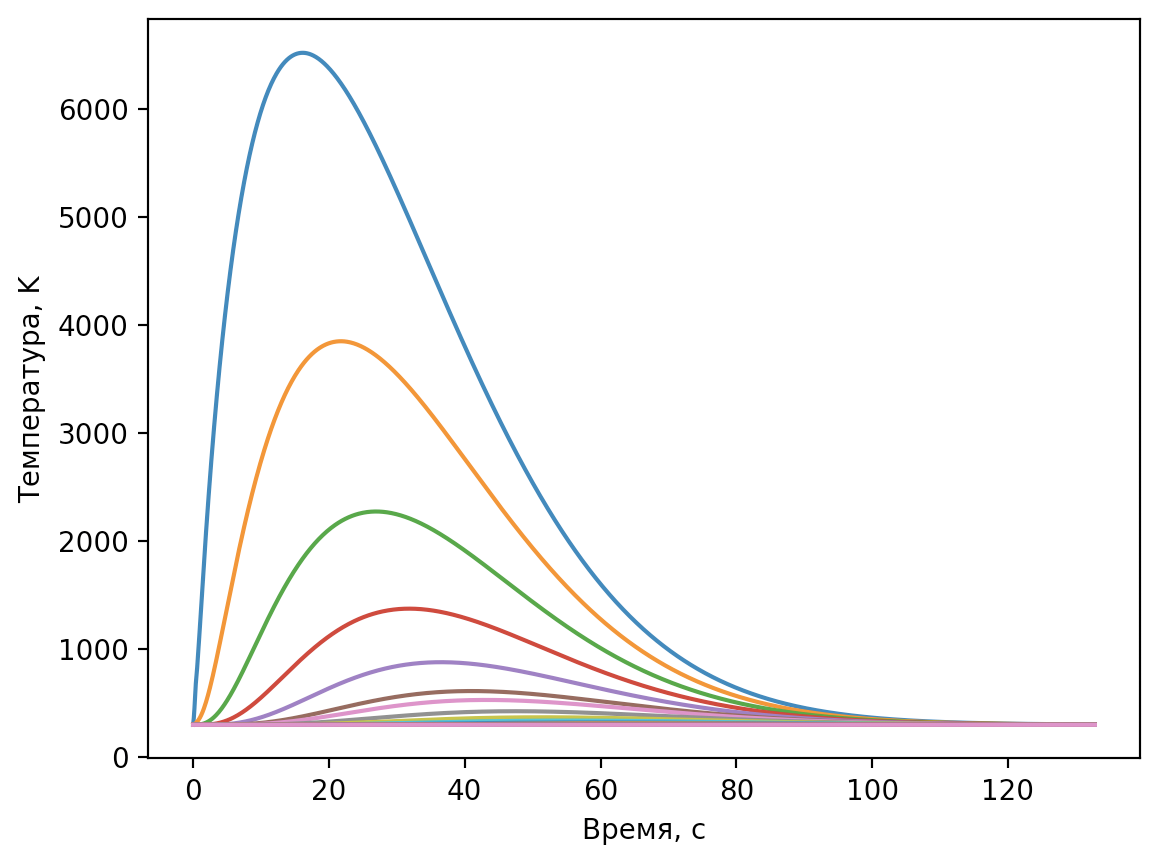
\includegraphics[scale=0.6]{5}

\newpage

$F_{max}=1000$

$t_{max}=100$ 

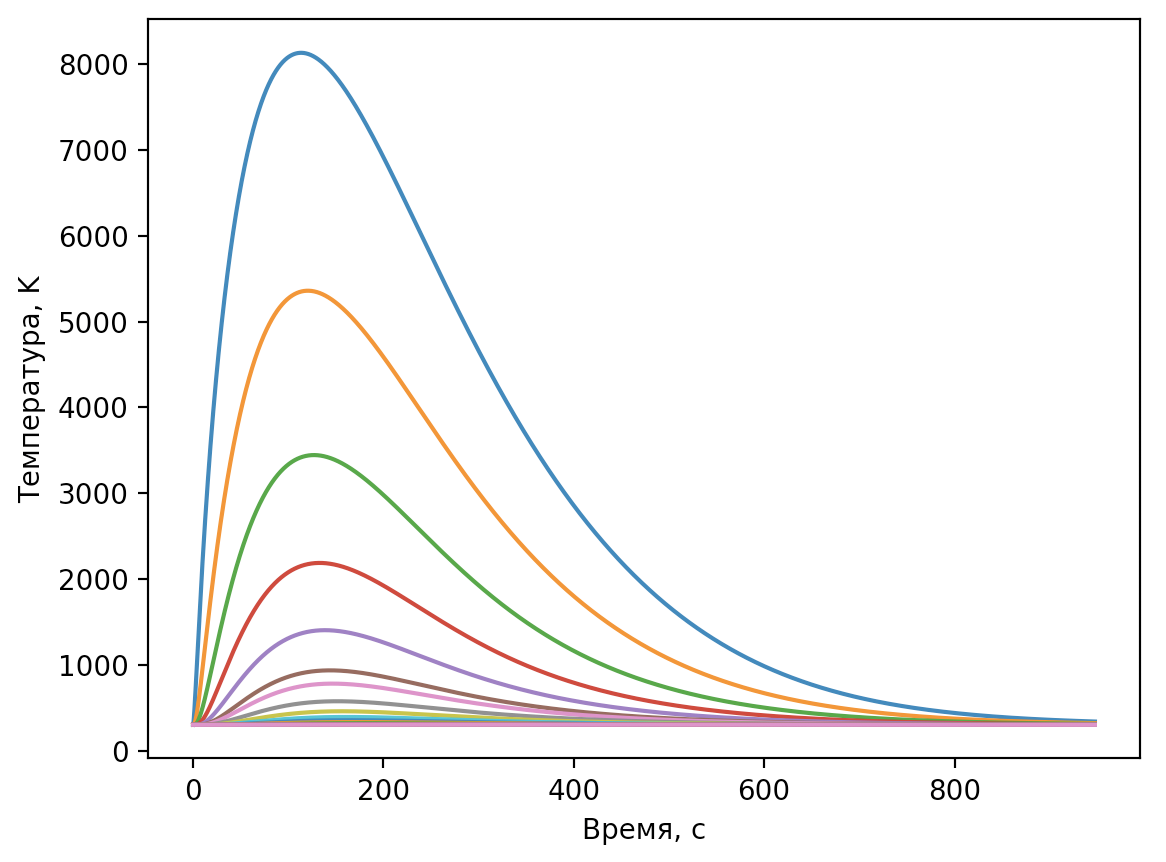
\includegraphics[scale=0.6]{6}

Таким образом, при увеличении $F_{max}$ возрастает и максимальная температура стержня. При изменении $t_{max}$ меняется время импульса, соответственно меняется время достижения точки с максимальной температурой. 

\newpage

\item График зависимости температуры при 3-4 значениях параметров $a_2, b_2$ теплоемкости. 

$a_2, b_2$ меняются попарно значениями из массивов:

$a_2=[0.5, 1, 2, 5]$

$b_2=[0.0005, 0.001, 0.005, 0.01]$

Соотвественно, с каждым шагом значение теплоемкости уведичивается. 

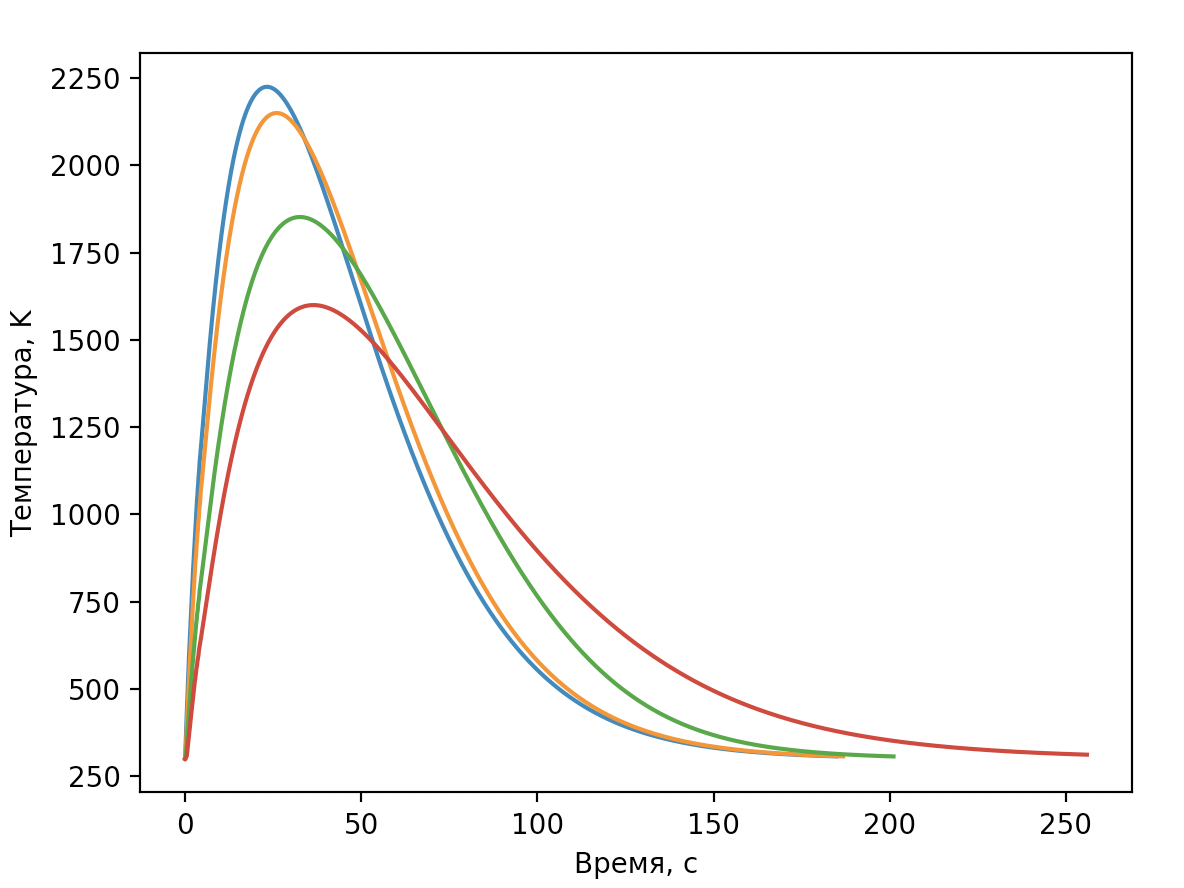
\includegraphics[scale=0.8]{7}

Графики по порядку:
\begin{itemize}
\item синий -- $a_2=0.5$, $b_2=0.0005$
\item оранжевый -- $a_2=1$, $b_2=0.001$
\item зеленый -- $a_2=2$, $b_2=0.005$
\item красный -- $a_2=5$, $b_2=0.01$
\end{itemize}

Получается, что с увеличением теплоемкости темп роста и максимальное значение температуры уменьшаются. 

\newpage

\item График зависимости температуры в частотном режиме теплового нагружения. Импульсы следуют один за другим с заданной частотой $\nu$ и длительностью $t_u$. 

\begin{itemize}
\item $\nu=\frac{1}{8}, t_u=4$

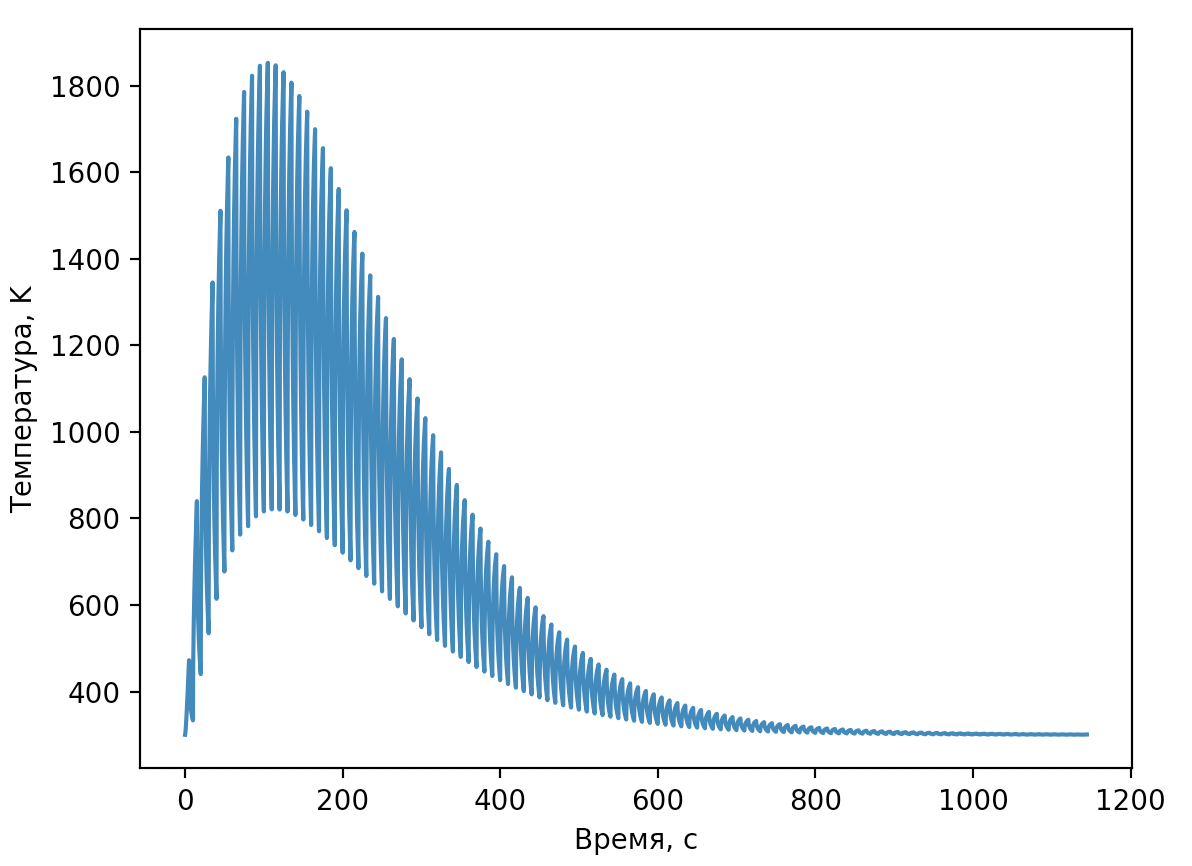
\includegraphics[scale=0.7]{8}

\newpage

\item $\nu=\frac{1}{5}, t_u=1$

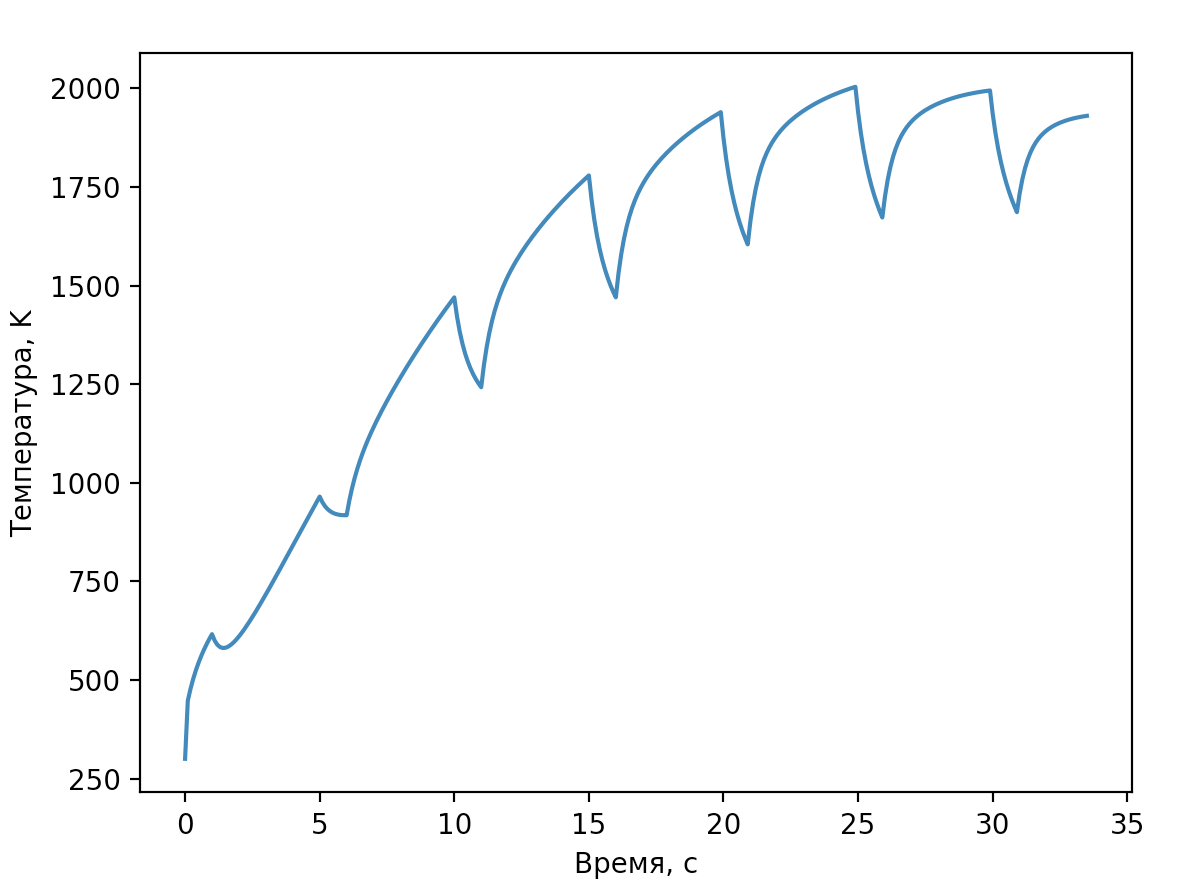
\includegraphics[scale=0.7]{9}

\item $\nu=\frac{1}{3}, t_u=1$

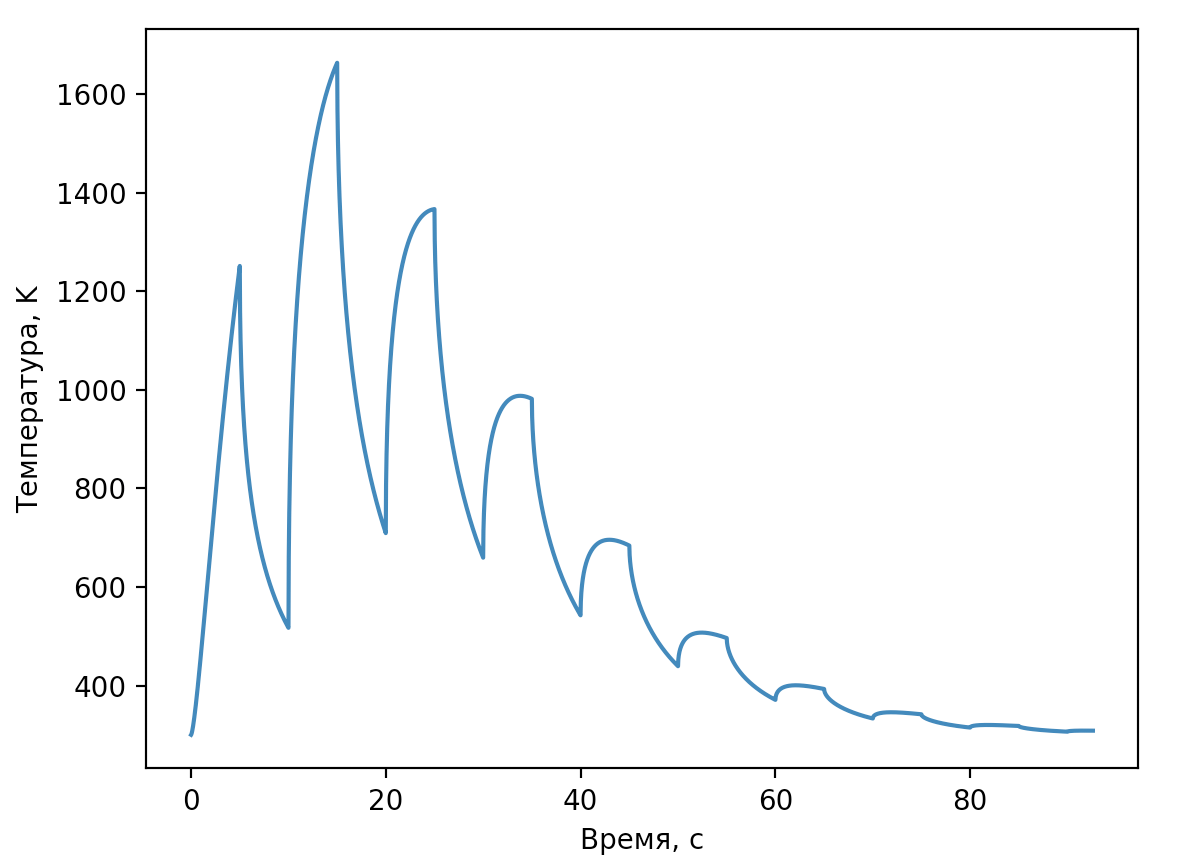
\includegraphics[scale=0.7]{10}

\end{itemize}

По мере роста частоты импульсов размах колебаний температуры уменьшается. 

Уменьшается вплоть до нуля в этот момент в торец поступает постоянный поток. 

Рассмотрим данный график и график из лабораторной работы 3 при всех одинаковых параметрах модели. 

\begin{figure}[ht]\center
	\begin{tabular}{cc}
		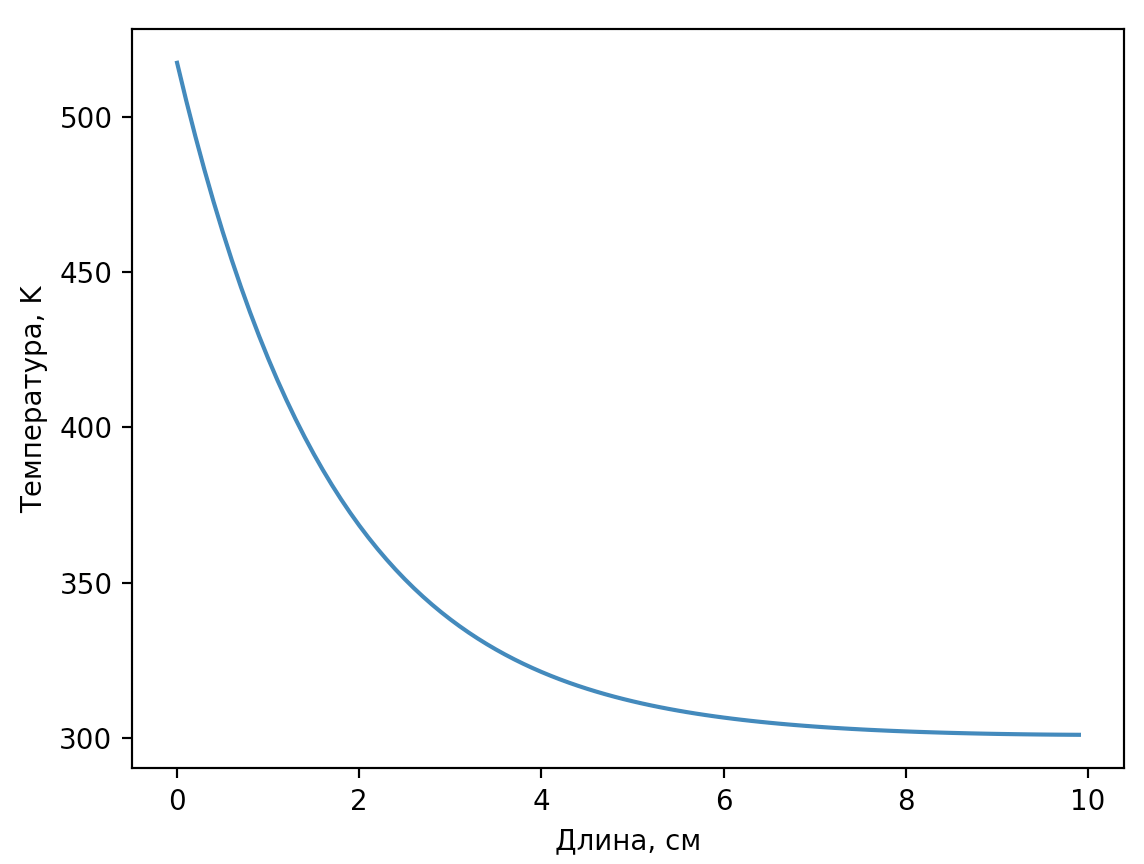
\includegraphics[width=90mm]{11} & 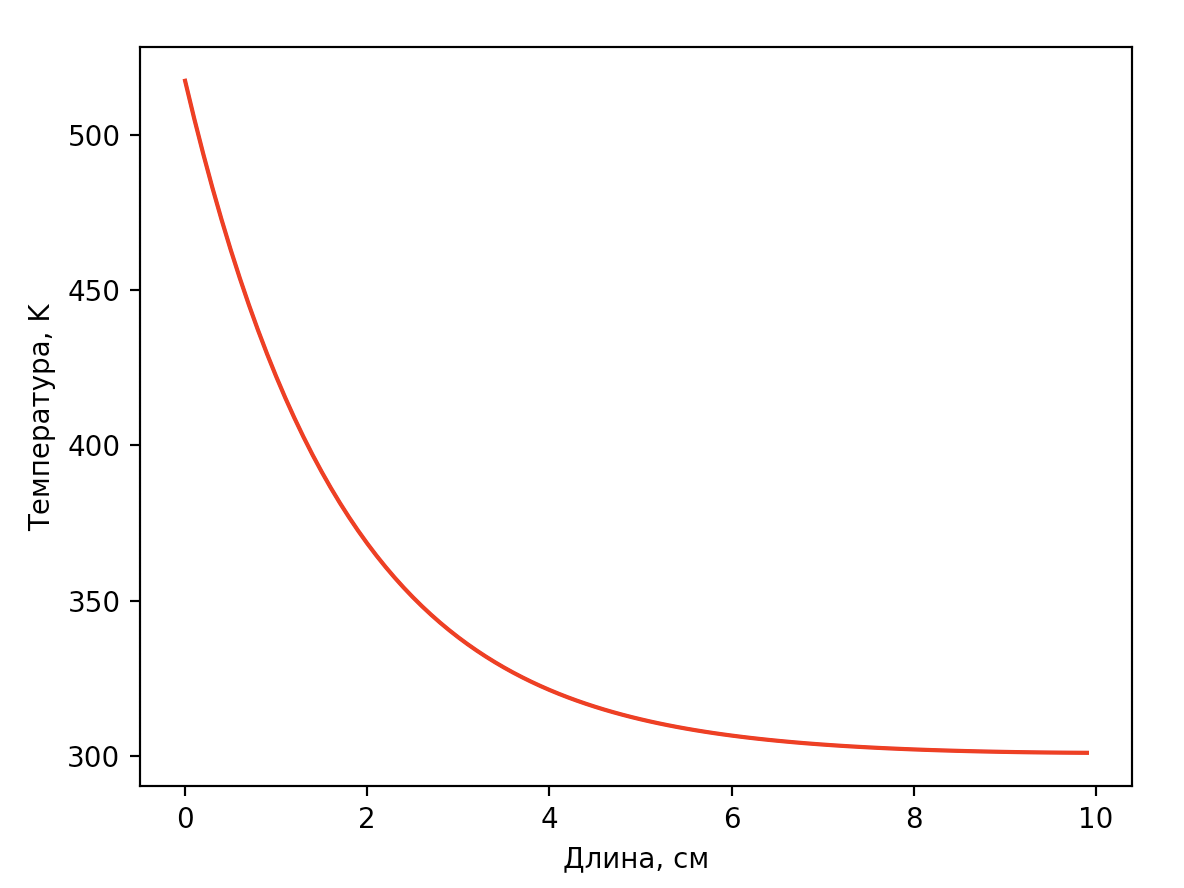
\includegraphics[width=90mm]{12}
	\end{tabular}
	\\ На левом рисунке представлен график из 3 работы, а на правом из текущей. 
\end{figure}

Полученное температурное поле совпало с результатом расчета $T(x)$. 

\end{enumerate}
\end{document}